%% UzK - A BEAMER THEME FOR THE UNIVERSITY OF COLOGNE
%% http://solstice.github.com/uzk-theme/

\documentclass[8pt]{beamer}

\usepackage{fontspec}

% Multilingual support
\usepackage{polyglossia}

% more symbols
\usepackage{textcomp}

% fontspec, realscripts, metalogo fot XeLaTeX
\usepackage{xltxtra}
	% Unicode fonts
	\setmainfont{CMU Serif}
	\setsansfont{CMU Sans Serif}
	\setmonofont{CMU Typewriter Text}
\usepackage{amsfonts}
\usepackage{unicode-math}
	\setmathfont{Latin Modern Math} % default
	\setmathfont{Latin Modern Math}[range={
		"1D608-"1D63B},	% Italic sans serif, Latin, uppercase
		sans-style=italic]
	\setmathfont{Latin Modern Math}[range={
		"1D6E2-"1D6FA,	% Italic Greek, uppercase
		"1D6FC-"1D71B},	% Italic Greek, lowercase
		math-style=ISO]
	\setmathfont{Latin Modern Math}[range={
		"00391-"003A9,	% Upright Greek, uppercase
		"003B1-"003F5,	% Upright Greek, lowercase
		"1D6A8-"1D6E1},	% Bold Greek
		sans-style=upright]
	\setmathfont{Asana Math}[range={
		\mathbin}] %\mathord
	\setmathfont{STIX Math}[range={
		"02609}] % ☉
	\setmathfont{XITS Math}[range={
		"1D4B6-"1D4CF}] % Script, Latin, lowercase
	%\setmathfont{⟨font name⟩}[range=⟨unicode range⟩,⟨font features⟩]

\usepackage{xeCJK}
\setmainlanguage{english}
\setotherlanguage{ngerman}

\usefonttheme{professionalfonts}
%  don't change fonts inside beamer

% AMS--related
\usepackage{amsmath,amssymb}

% ':=' as \coloneqq
\usepackage{mathtools}
\usepackage{siunitx}
\usepackage{cleveref}
\usepackage{booktabs}

% some unicode characters
% ≙ for equal with hat


% Mathematical constants
\newcommand{\ii}{{\Bbbi}}
\newcommand{\ee}{{\Bbbe}}
\newcommand{\pp}{{\Bbbpi}}

% Math operators
\DeclareMathOperator{\arcsinh}{arcsinh}
\DeclareMathOperator{\arccosh}{arccosh}
\DeclareMathOperator{\arctanh}{arctanh}
\DeclareMathOperator{\arccoth}{arccoth}
\DeclareMathOperator{\arcctgh}{arcctgh}
\DeclareMathOperator{\arcsech}{arcsech}
\DeclareMathOperator{\arccsch}{arccsch}

\DeclareMathOperator{\BesselJ}{J}
\DeclareMathOperator{\BesselY}{Y}
\DeclareMathOperator{\BesselF}{F}
\DeclareMathOperator{\BesselG}{G}
\DeclareMathOperator{\BesselI}{I}
\DeclareMathOperator{\BesselK}{K}
\DeclareMathOperator{\BesselL}{L}

\DeclareMathOperator{\sgn}{sgn}
\DeclareMathOperator{\grad}{grad}
\DeclareMathOperator{\curl}{curl}
\DeclareMathOperator{\rot}{rot}
\DeclareMathOperator{\opdiv}{div}
\DeclareMathOperator{\opdeg}{deg}

\DeclareMathOperator{\sech}{sech}
\DeclareMathOperator{\csch}{csch}

\DeclareMathOperator{\diag}{diag}
\DeclareMathOperator{\tr}{tr}
\DeclareMathOperator{\rank}{rank}

\DeclareMathOperator{\ad}{ad}

\DeclareMathOperator{\expi}{expi}

% Differentials
\newcommand{\DD}{\BbbD}
\newcommand{\dd}{\Bbbd}
\newcommand{\dva}{\mupdelta} % no better way?!
\newcommand{\Dva}{\mupDelta}

% Equal marks
\newcommand{\eeq}{{\overset{!}{=}}}
\newcommand{\lls}{{\overset{!}{<}}}
\newcommand{\ggt}{{\overset{!}{>}}}
\newcommand{\lle}{{\overset{!}{\le}}}
\newcommand{\gge}{{\overset{!}{\ge}}}

% Group and Algebras
\newcommand{\SO}{\msansS\msansO}
\newcommand{\SU}{\msansS\msansU}
\newcommand{\so}{\mfraks\mfrako}
\newcommand{\su}{\mfraks\mfraku}
% Bracket-like
\newcommand{\rbr}[1]{{\left(#1\right)}}
\newcommand{\sbr}[1]{{\left[#1\right]}}
\newcommand{\cbr}[1]{{\left\{#1\right\}}}
\newcommand{\abr}[1]{{\left<#1\right>}}
\newcommand{\vbr}[1]{{\left|#1\right|}}
\newcommand{\dvbr}[1]{{\left\|#1\right\|}}
\newcommand{\fat}[2]{{\left.#1\right|_{#2}}}
% Functions; note the space between the name and the bracket!
\newcommand{\rfun}[2]{{#1}\mathopen{}\left(#2\right)\mathclose{}}
\newcommand{\sfun}[2]{{#1}\mathopen{}\left[#2\right]\mathclose{}}
\newcommand{\cfun}[2]{{#1}\mathopen{}\left\{#2\right\}\mathclose{}}
\newcommand{\afun}[2]{{#1}\mathopen{}\left<#2\right>\mathclose{}}
\newcommand{\vfun}[2]{{#1}\mathopen{}\left|#2\right|\mathclose{}}
% Fraction-like
\newcommand{\frde}[2]{{\frac{\dd{#1}}{\dd{#2}}}}
\newcommand{\frDe}[2]{{\frac{\DD{#1}}{\DD{#2}}}}
\newcommand{\frpa}[2]{{\frac{\partial{#1}}{\partial{#2}}}}
\newcommand{\frdva}[2]{{\frac{\dva{#1}}{\dva{#2}}}}

% overline-like marks
\newcommand{\ol}[1]{{\overline{{#1}}}}
\newcommand{\ul}[1]{{\underline{{#1}}}}
\newcommand{\tld}[1]{{\widetilde{{#1}}}}
\newcommand{\ora}[1]{{\overrightarrow{#1}}}
\newcommand{\ola}[1]{{\overleftarrow{#1}}}
\newcommand{\td}[1]{{\widetilde{#1}}}
\newcommand{\what}[1]{{\widehat{#1}}}
%\newcommand{\prm}{{\symbol{"2032}}}

% Physical constants and parameters
\newcommand{\lc}{\mitsansc} % speed of light in vacuum
\newcommand{\bk}{\mitsansk} % Boltzmann's constant
\newcommand{\phs}{\hslash} % reduced Planck constant
\newcommand{\ph}{\Planckconst} % Planck constant

\newcommand{\nG}{\mitsansG} % Newton's constant
\newcommand{\aN}{\mitsansN} % Avogadro number
\newcommand{\ec}{\mitsanse} % unit electric charge

\newcommand{\gR}{\mitsansR} % gas constant

\newcommand{\plm}{m_\text{P}} % Planck mass
\newcommand{\pll}{l_\text{P}} % Planck length
\newcommand{\plt}{t_\text{P}} % Planck time

\newcommand{\hH}{\mitsansH} % Hubble parameter H
\newcommand{\hh}{\mitsansh} % Hubble parameter h
\newcommand{\dq}{\mitsansq} % Deceleration parameter q

\newcommand{\apE}{\alpha_\text{E}} % EM fine struct const
\newcommand{\apG}{\alpha_\text{G}} % Grav fine struct const

% Common symbols
\newcommand{\Ld}{\mscrL} % Lagrangian density
\newcommand{\fp}{p_\text{F}} % Fermi momentum
\newcommand{\fE}{\mscrE_\text{F}} % Fermi energy

% Others
\newcommand{\rSch}{R_\text{S}} % Schwarzschild radius

\newcommand{\fHor}{{\mscrh^+}} % future horizon
\newcommand{\pHor}{{\mscrh^-}} % past horizon

% Chemical elements
\usepackage[version=4]{mhchem}


% siunitx
% Astronomy
\DeclareSIUnit\parsec{pc}
\DeclareSIUnit\lightyear{ly}

\usepackage[style=science,
			firstinits=true,
			isbn = false, doi = false,
			backend=biber]{biblatex}
\addbibresource{../liouville-cosmology.bib}
%\AtEveryBibitem{
%		\clearfield{issn}
%		\clearfield{month}
%		\clearfield{url}
%		\clearfield{publisher}
%		\clearfield{series}
%		\clearfield{volume}
%	\ifentrytype{book}{
%		\clearfield{publisher}
%	}{
%		\clearfield{title}
%	}
%}
%\AtEveryCitekey{
%		\clearfield{issn}
%		\clearfield{month}
%		\clearfield{url}
%		\clearfield{publisher}
%		\clearfield{series}
%		\clearfield{volume}
%	\ifentrytype{book}{
%		\clearfield{publisher}
%	}{
%		\clearfield{title}
%	}
%}

%% Falls Anzeige der \sections, \subsections etc. gewuenscht, kann zB.
%% das infolines theme geladen werden. Wichtig ist jedoch, dass andere
%% Themes _vor_ dem UzK-Theme geladen werden.
%\useoutertheme{infolines}

%% Falls keine der Optionen zur Bestimmung der Fusszeile uebergeben werden    %%
%% werden alle Fakultaetsfarben verwendet. ---------------------------------- %%
\usetheme[%
%wiso,        %% Wiso-Fakultaet
%jura,        %% Rechtswissenschaftliche Fakultaet
%medizin,     %% Medizinische Fakultaet
%philo,       %% Philosophische Fakultaet
%matnat,      %% Mathematisch-Naturwissenschaftliche Fakultaet
%human,       %% Humanwissenschaftliche Fakultaet
%verw,        %% Universitaetsverwaltung
%nav,         %% Schaltet die Navigationssymbole ein
latexfonts,  %% Verwendet die latex-beamer-Standardschrift
colorful,    %% Farbige Balken im infolines-Theme
%squares,     %% Aufzaehlungspunkte rechteckig
%nologo,      %% Kein Logo im Seitenhintergrund
]{UzK}

\title{Integrable Liouville Cosmological Models}
\subtitle{Self-adjointness of the Hamiltonian and Semi-classical Wave Functions}

\date{March 23, 2018}

\author[Andrianov \and Lan \and Novikov \and \underline{Wang}]{
	Alexander A. Andrianov\inst{1,4} %\thanks{a.andrianov@spbu.ru}
	\and
	Chen Lan\inst{2} %\thanks{stlanchen@yandex.ru}
	\and
	Oleg O. Novikov\inst{1} %\thanks{o.novikov@spbu.ru}
	\and 
	\underline{Yi-Fan Wang}\inst{3}} %\thanks{yfwang@thp.uni-koeln.de}
%{David Kusterer\thanks{ 
%\href{mailto:kusterer@uni-koeln.de}{kusterer@uni-koeln.de} }%
%  \and%
%  Bernd 
%Weiß\thanks{\href{mailto:bernd.weiss@wiso.uni-koeln.de}{
%bernd.weiss@wiso.uni-koeln.de}}}

%\institute[Forschungsinstitut für Soziologie]{%
%Forschungsinstitut für Soziologie \\
%Greinstraße 2\\
%50939 Köln}

\institute[SPBU \and ELI-ALPS \and UzK \and UB]{
\inst{1} Saint-Petersburg State University,
Ulyanovskaya str. 1, Petrodvorets, Sankt-Petersburg 198504, Russland
\and
\inst{2}
ELI-ALPS Research Institute,
Budapesti út 5, H-67228 Szeged, Ungarn
\and
\inst{3}
Institut für Theoretische Physik, Universität zu Köln,
Zülpicher Straße 77, D-50937 Köln, Deutschland
\and
\inst{4}
Institut de Ciències del Cosmos, Universitat de Barcelona, Martí i Franquès 1, 
E-08028 Barcelona, Spanien}

\AtBeginSection[]
{
 \begin{frame}<beamer>
 \frametitle{Outline}
 \tableofcontents[currentsection]
 \end{frame}
}

\begin{document}

\begin{frame}%[titlepage]
  \titlepage
\end{frame}

\begin{frame}{Outline}
  \tableofcontents
  % You might wish to add the option [pausesections]
\end{frame}


\section{Introduction}

\begin{frame}%
{Introduction}%
{The Friedmann--Lemaître model with quintessence and phantom Liouville fields}
\begin{itemize}
%\item Observed accelerated expansion can be explained by a cosmological 
%constant\footfullcite{COPELAND2006,Bamba2012} as stationary Dark Energy, but 
%its %origin has yet to be understood.

\item Dynamical Dark Energy has been modelled by
quintessence\footfullcite{Caldwell1998} and phantom\footfullcite{Caldwell2002} 
matter, %with barotropic index\footnote{Barotropic index is the $w$ in equation
%of state $\rho = wp$.} $w > -1$ and $w < -1$, respectively.
%
%\item They
which can be realised by minimally-coupled real scalar fields with 
\textcolor{blue}{$\mscrl = \pm 1$}\footnote{The signature of metric is $\rbr{-, 
+, \ldots, +}$.}
\begin{align}
\mscrS_{\text{L}} = \int\dd^4 x\,\sqrt{-g}\,\cbr{-\mscrl \frac{g^{\mu\nu}}{2}
\rbr{\partial_\mu\phi}\rbr{\partial_\nu\phi} - \rfun{\mscrV}{\phi}}.
\end{align}

\item The Liouville field\footfullcite{NAKAYAMA2004} $\rfun{\mscrV}{\phi} =
V\ee^{\lambda\phi}$ is of interest, where $\lambda, V\in \BbbR$.

\item Assume a flat Robertson--Walker metric $g_{\mu\nu}\,\dd x^\mu\,\dd x^\nu
= -\rfun{N^2}{t}\,\dd t^2
+ \varkappa \ee^{2\rfun{\alpha}{t}}\,\dd\Omega_{3\text{F}}^2$, where
$\varkappa \coloneqq 8\pp\nG$,
$\dd\Omega_{3\text{F}}^2 \coloneqq
\dd\chi^2+\chi^2\rbr{\dd\theta^2+\sin^2\theta\,\dd\varphi^2}$, and
$N$ lapse function.

\item The total action reads
$\mscrS \coloneqq \mscrS_{\text{EH}} + \mscrS_\text{GHY} + \mscrS_\text{L}
= \int\dd\Omega_{3\text{F}}^2\int\dd t\,L$, where
\begin{align}
L&\coloneqq \varkappa^{3/2}N\ee^{3\alpha}
\rbr{-\frac{3}{\varkappa}\frac{\dot{\alpha}^2}{N^2}
+\mscrl\frac{\dot{\phi}^2}{2N^2}-V\ee^{\lambda\phi}}.
\label{eq:eff-lag-10}
\end{align}

\end{itemize}
\end{frame}

\begin{frame}%
{Introduction}%
{Highlights}
\begin{block}{Integrability}
With the help of an integral of motion, implicit trajectories can be obtained 
explicitly, and the minisuperspace Wheeler--DeWitt equation can be integrated 
exactly.
\end{block}

\begin{block}{Self-adjointness}
Imposing self-adjointness of the Hamiltonian leads to removal of the degeneracy 
and discretisation of the spectrum.
\end{block}

\begin{block}{Semi-classical wave functions}
Semi-classical wave functions can be constructed by the principle of
constructive interference, the Wentzel--Kramers--Brillouin approximation and
numerical methods.
\end{block}

\end{frame}

\section{The classical model and the implicit trajectories}

\subsection{Lagrangian formalism and the first integral}

\begin{frame}%
{Decoupling the variables}%
{Via orthogonal transformation}
\begin{itemize}
\item By rescaling $\overline{N} \coloneqq N\ee^{-3\alpha}$ and
%\item Setting $\overline{N} \coloneqq N\ee^{-3\alpha}$, \cref{eq:eff-lag-10}
%%the effective Lagrangian
%transforms to
%\begin{align}
%L = \varkappa^{3/2}\overline{N}
%\rbr{-\frac{3}{\varkappa}\frac{\dot{\alpha}^2}{\overline{N}^2}
%+\mscrl\frac{\dot{\phi}^2}{2\overline{N}^2} - V\ee^{\lambda\phi+6\alpha}}
%\end{align}
%
%\item Defining $\Delta \coloneqq \lambda^2 - 6\mscrl\varkappa$,
%$\mscrs \coloneqq \sgn \Delta$ and
%$g \coloneqq \mscrs \sqrt{\vbr{\Delta}} \equiv \mscrs\sqrt{\mscrs\Delta}$,
the orthogonal transformation
\begin{align}
\begin{pmatrix}
\rfun{\alpha}{t} \\ \rfun{\phi}{t}
\end{pmatrix} = \frac{\mscrs}{g}
\begin{pmatrix}
\lambda & -\mscrl\varkappa \\
-6 & \lambda
\end{pmatrix}
\begin{pmatrix}
%\mscrs_\beta \cdot \rfun{\beta}{t} \\ \mscrs_\chi \cdot \rfun{\chi}{t}
\rfun{\beta}{t} \\ \rfun{\chi}{t}
\end{pmatrix},
%\qquad\text{where } \mscrs_\beta, \mscrs_\chi = \pm 1,
\end{align}
the system can be decoupled
%($\mscrs_\beta = \mscrs_\chi = +1$ from now on)
%gives the decoupled Lagrangian
($\Delta \coloneqq \lambda^2 - 6\mscrl\varkappa$,
\textcolor{blue}{$\mscrs \coloneqq \sgn \Delta$} and
$g \coloneqq \mscrs \sqrt{\vbr{\Delta}} \equiv \mscrs\sqrt{\mscrs\Delta}$)
\begin{align}
L = \varkappa^{3/2}\overline{N}
\rbr{-\mscrs\frac{3}{\varkappa}\frac{\dot{\beta}^2}{\overline{N}^2}
+\mscrl\mscrs\frac{\dot{\chi}^2}{2\overline{N}^2}
-V\ee^{g \chi}}.
\label{eq:lagrangian-decoupled}
\end{align}

%\item
%The Euler--Lagrange equations with respect to $\overline{N}$, $\beta$ and
%$\chi$ will be called the modified first, second Friedmann equations and the
%Klein--Gordon equation, respectively.

\item Using the \alert{conservation of $p_\beta$}\footfullcite[The same 
first integral has been found in][in canonical 
formalism]{Lan2016,Andrianov2015}, $\rfun{\overline{N}}{t}$ can be eliminated, 
leading to the exact integrations of the equations of motion as \alert{implicit 
trajectories}.
\begin{itemize}
\item $p_\beta \neq 0$: four cases according to $\rbr{\mscrl, \mscrs \mscrv}$,
\textcolor{blue}{$\mscrv \coloneqq \sgn V$}.
\item $p_\beta = 0$: well-known power-law special solution for $\rbr{+,-}$ 
and $\rbr{-,+}$.
\end{itemize}

\end{itemize}
\end{frame}


\begin{frame}%
{Trajectories for quintessence model $\rbr{+,+}$}%
{$\sech$, with $\beta_0 = 0$, $\vbr{V} = \varkappa^{-2}$ and
$p_\beta^2 = \varkappa^2\sqrt{\vbr{V}}$; varying $\lambda$}

\begin{align}
\ee^{g\textcolor{red}{\chi}} = 
\tfrac{p_\beta^2}{12\varkappa^2\vbr{V}}
\rfun{\sech^2}{ \sqrt{\tfrac{3}{2\varkappa}}\,g 
\rbr{\textcolor{red}{\beta}-\beta_0}}
\end{align}
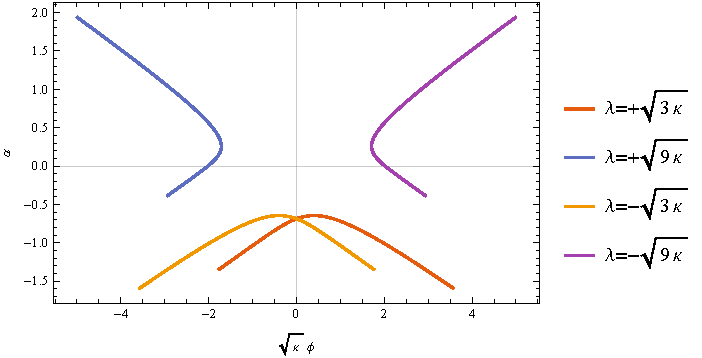
\includegraphics[width=\textwidth]{../plots.nb/sech_lamb.pdf}

\end{frame}


\begin{frame}%
{Trajectories for quintessence model $\rbr{+,-}$}%
{$\csch$, with $\beta_0 = 0$, $\vbr{V} = \varkappa^{-2}$ and
$p_\beta^2 = \varkappa^2\sqrt{\vbr{V}}$; varying $\lambda$}
\begin{align}
\ee^{g\textcolor{red}{\chi}} = 
\tfrac{p_\beta^2}{12\varkappa^2\vbr{V}}
\rfun{\csch^2}{ \sqrt{\tfrac{3}{2\varkappa}}\,g 
\rbr{\textcolor{red}{\beta}-\beta_0}}
\end{align}
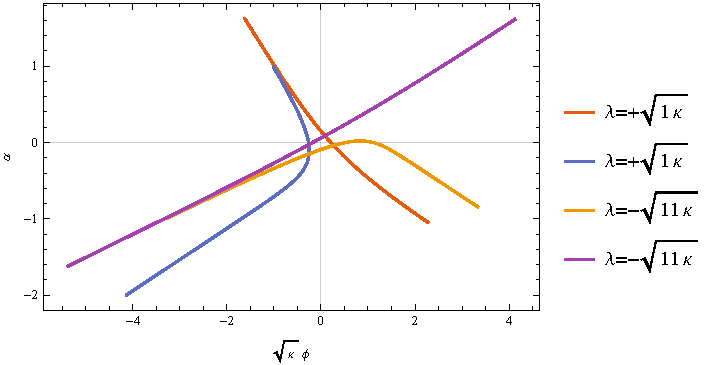
\includegraphics[width=\textwidth]{../plots.nb/csch_lamb_l.pdf}

\end{frame}


\begin{frame}%
{Trajectories for phantom model $\rbr{-,+}$}%
{$\sec$, with $V = \varkappa^{-2}$ and
$p_\beta^2 = 3\varkappa^2\sqrt{\vbr{V}}$}
\begin{align}
\ee^{g\textcolor{red}{\chi}} = 
\tfrac{p_\beta^2}{12\varkappa^2\vbr{V}}
\rfun{\sec^2}{ \sqrt{\tfrac{3}{2\varkappa}}\,g 
\rbr{\textcolor{red}{\beta}-\beta_0}}
\end{align}
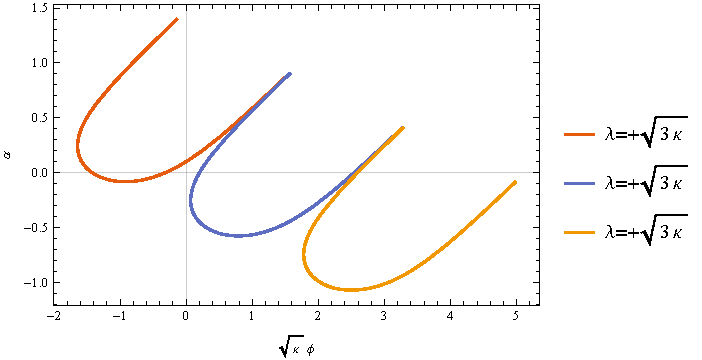
\includegraphics[width=\textwidth]{../plots.nb/csc_lamb_l.pdf}

\end{frame}

\section{Dirac quantisation and self-adjointness of the Hamiltonian}

\subsection{Dirac quantisation and the quantum-mechanical analogy}

\begin{frame}%
{Dirac quantisation}%
%{233}
\begin{itemize}
\item
The primary Hamiltonian and the Hamiltonian
constraint\footfullcite{Gitman1990,Rothe2010} reads
\begin{align}
H^\text{p} &= \overline{N}H_\perp + v^{\overline{N}} p_{\overline{N}},
\\
H_\perp &\coloneqq -\mscrs\frac{p_\beta^2}{12\varkappa^{1/2}}
+\mscrl\mscrs\frac{p_\chi^2}{2\varkappa^{3/2}}
+\varkappa^{3/2}V\ee^{g\chi}.
\end{align}
\item
Applying the Dirac quantisation rules with the Laplace--Beltrami
operator ordering\footfullcite[ch.\ 8]{Kiefer2012}, one 
gets the minisuperspace Wheeler--DeWitt equation with $\rbr{\beta,\chi}$
%$\widehat{H}_\perp \rfun{\Psi}{\beta,\chi} = 0$,
\begin{align}
% -\mscrs \frac{12\varkappa^{1/2}}{\hslash^2}\widehat{H}_\perp 
% \Psi \eqqcolon -\partial_\beta^2\Psi - \BbbD\Psi,\qquad
% \BbbD = -\mscrl \frac{6}{\varkappa}\partial_\chi^2 +
% \mscrs \frac{12\varkappa^2 V \ee^{g\chi}}{\hslash^2}.
0 &= \widehat{H}_\perp \rfun{\Psi}{\beta,\chi} \coloneqq
\rbr{\mscrs\frac{\hslash^2}{12\varkappa^{1/2}}\partial_{\beta}^2
-\mscrl\mscrs\frac{\hslash^2}{2\varkappa^{3/2}}\partial_{\chi}^2
+\varkappa^{3/2}V\ee^{g \chi}}\Psi.
\label{eq:WDW-10}
\end{align}
\item
\Cref{eq:WDW-10} is Klein--Gordon-like, hyperbolic for $\mscrl = +1$ and 
\emph{elliptic} for $\mscrl = -1$.
\end{itemize}
\end{frame}

\begin{frame}%
{Integration of the Wheeler--DeWitt equation}%
{The quantum-mechanical analogy}
\begin{itemize}
\item Fourier transforming $\beta$ to $k_\beta \in \BbbR$ yields the
time-independent Schr\"odinger equation
\begin{align}
E \rfun{\psi}{x} \coloneqq
\mscrl \frac{\hslash^2\widetilde{g}^2\nu^2}{8\mitsansM_\text{P}} \psi
= \widehat{H}_\text{eff} \psi \coloneqq
\rbr{-\frac{\hslash^2}{2 \mitsansM_\text{P}} \partial_x^2
+ V_{\text{eff}}} \psi,\quad
V_{\text{eff}} \coloneqq
\mscrl \mscrs \mscrv \widetilde{V} \ee^{\widetilde{g} x},
\end{align}
in which $\mitsansM_\text{P} \coloneqq \sqrt{\frac{\hslash}{\varkappa}}$,
$x \coloneqq \sqrt{\hslash}\varkappa\cdot\chi$,
$\widetilde{V} \coloneqq \mitsansM_\text{P}^{-3} \vbr{V} \ge 0$, and
$\nu = \sqrt{\frac{2\varkappa}{3}} \frac{\vbr{k_\beta}}{g} \ge 0$.
%, and $\widetilde{g} \coloneqq \varkappa^{-1} g$.
\begin{itemize}
\item The Liouville potential $V_{\text{eff}}$ is a special case of the Morse
potential\footfullcite{Morse1929,Gitman2012}.
\item The Starobinsky model in the Einstein frame is related to the Morse 
potential.
\end{itemize}

\item Let $\ee^{2y} \coloneqq
8\mitsansM_{\text{P}}\widetilde{V}/\hslash^2\widetilde{g}^2\cdot
\ee^{\widetilde{g}x}$; there are four cases according to $\rbr{\mscrl, \mscrs 
\mscrv}$, and the mode functions are
%\item For the quintessence model $\rbr{+, +}$:
%$V_{\text{eff}}$ is bounded \textcolor{blue}{below};
%generalised eigenfunctions are the Besselian
%$\rfun{\BesselK_{\ii \nu}}{\ee^{\widetilde{x}}}$'s, $\ee^{2\widetilde{x}} =
%8\mitsansM_{\text{P}}\widetilde{V}/\hslash^2\widetilde{g}^2\cdot
%\ee^{\widetilde{g}x}$.

%\item For the quintessence model  $\rbr{+, -}$:
%$V_{\text{eff}}$ is bounded \alert{above}; generalised eigenfunctions 
%for positive spectrum (scattering states) are the Besselian
%$\rfun{\BesselF_{\ii \nu}}{\ee^{\widetilde{x}}}$'s and
%$\rfun{\BesselG_{\ii \nu}}{\ee^{\widetilde{x}}}$'s\footfullcite[These are
%linear combinations of $\rfun{\BesselJ_{\pm\ii \nu}}{\ee^{\widetilde{x}}}$;
%see][]{Dunster1990}.

%\item For the phantom model $\rbr{-, +}$:
%$V_{\text{eff}}$ is bounded \alert{above}; eigenfunctions 
%for negative eigenvalues (bound states) are the Besselian
%$\rfun{\BesselJ_{\nu}}{{\ee^{\widetilde{x}}}}$'s.
\end{itemize}

\begin{center}
\begin{tabular}{c||r@{; }l|r@{; }l}
\toprule
& \multicolumn{2}{c}{$E \ge 0$} & \multicolumn{2}{|c}{$E < 0$} \\
\midrule
$V_{\text{eff}}\,\textcolor{blue}{>}\,0$ &
$\rbr{+,+}$ & $\rfun{\BesselK_{\ii \nu}}{\ee^{y}}$ &
$\rbr{-,-}$ & none \\
$V_{\text{eff}}\,\textcolor{red}{<}\,0$ &
$\rbr{+,-}$ &
$\rfun{\BesselF_{\ii \nu}}{\ee^{y}}$,
$\rfun{\BesselG_{\ii \nu}}{\ee^{y}}$ &
$\rbr{-,+}$& $\rfun{\BesselJ_{\nu}}{\ee^{y}}$ \\
\bottomrule
\end{tabular}
\end{center}

\end{frame}

\subsection{Self-adjointness of the Hamiltonian}

\begin{frame}%
{Self-adjointness of the Hamiltonian}%
{Results for the Liouville potential\footfullcite[See 
also][sec.~8.5]{Gitman2012}}
\begin{itemize}
\item $k_\beta \in \BbbR$, enforcing the self-adjointness of 
$\widehat{H}_{\text{eff}}$.

\item For $V_{\text{eff}} > 0$: $\widehat{H}_\text{eff}$ is
\textcolor{blue}{essentially self-adjoint}%
\footfullcite[See also][sec.~9.9]{hall2013}.
\begin{itemize}
\item Quintessence $\rbr{+, +}$: nothing special.
\end{itemize}

\item For $V_{\text{eff}} < 0$: $\widehat{H}_\text{eff}$ admits
\textcolor{orange}{a family of self-adjoint extensions}.
\begin{itemize}
\item Quintessence $\rbr{+,-}$: ``eigenfunctions'' are
linear combinations of $\BesselF$ and $\BesselG$;
\alert{the degeneracy is removed}
\item Phantom $\rbr{-, +}$: the spectrum becomes \alert{discrete}
\begin{align}
\rfun{\psi_{-+,\nu}}{\ee^y} &\propto
\rfun{\BesselJ_{\nu}}{\ee^y},\qquad \nu = 2n+a_<,\, \alert{n \in
\BbbZ_\ge},
\label{eq:Phi_nu}
\end{align}
and the corresponding full wave-functions are Bloch-periodic.
%$\rfun{\Psi_{-+,n}}{\beta,\chi} = \ee^{\ii\pp a_<}
%\rfun{\Psi_{-+,n}}{\beta + T_\beta,\chi}$.
Imposing (anti-)periodic boundary condition fixes $a_< = 0$ ($1$).
\end{itemize}

%\item For $\rbr{+, -}$ and $\rbr{-, +}$:
%$\widehat{H}_\text{eff}$ is \alert{not self-adjoint} but admits a family of
%self-adjoint extensions parametrised by $a \in [0,2)$.

%\item For the quintessence model $\rbr{+,-}$, the generalised eigenfunctions are
%\begin{align}
%{}_{\rbr{+,-}}\psi_\nu &\propto \BesselF_{\ii\nu}\cos\frac{\pp a_\ge}{2}
%+ \BesselG_{\ii\nu}\sin\frac{\pp a_\ge}{2}
%\end{align}
%with asymptotic behaviour $\rfun{{}_{\rbr{+,-}}\psi_\nu}{\ee^{\widetilde{x}}}
%\sim \ee^{-\widetilde{x}/2}
%\rfun{\cos}{\ee^{\widetilde{x}}-\frac{\pp a}{2}-\frac{\pp}{4}}$
%as $x \to +\infty$.


%\begin{itemize}
%\item \Cref{eq:Phi_nu} can also be shown by noting
%$\rbr{\BesselJ_{\mu}, \widehat{H}_{\text{eff}} \BesselJ_{\nu}}_\text{S} - 
%\rbr{\widehat{H}_{\text{eff}} \BesselJ_{\mu}, \BesselJ_{\nu}}_\text{S} \propto
%\sin \frac{\pp\rbr{\mu-\nu}}{2}$
%and then imposing symmetricity.

%\item 
%\end{itemize}

\item The self-adjointness has been discussed in quantum cosmology in e.g.\
\footfullcite{Almeida2015} (operator ordering) and more 
recently in \footfullcite{Gryb2018} ($\Lambda$ as a quantum number).

\end{itemize}

\end{frame}


%\begin{frame}%
%{The self-adjointness of the Hamiltonian}%
%{Discussion}%
%{233}

%\begin{itemize}
%\item The self-adjointness of $\widehat{H}_\text{eff}$ is non-trivial and not
%unique for $\rbr{+, -}$ and $\rbr{-, +}$.

%\item For the phantom model $\rbr{-, +}$, it \alert{discretises} the spectrum.

%\item The self-adjointness has been discussed in quantum cosmology in e.g.\
%\footfullcite{Almeida2015} (in the operator ordering scenario) and more 
%recently in \footfullcite{Gryb2018}.

%\item The self-adjoint extension is also non-trivial for the $x^{-2}$
%potential\footfullcite{Essin2006}, which is of cosmological relevance as well%
%\footfullcite{Bouhmadi-Lopez2009}.
%\end{itemize}

%\end{frame}



\section{The semi-classical wave functions}

\subsection{The Wentzel--Kramers--Brillouin approximation}

\begin{frame}%
{Matching quantum number with classical first integral}%
{Principle of constructive interference; $\rbr{+,+}$ as the example}

\begin{itemize}
\item Write the mode function in the Wentzel--Kramers--Brillouin form
$\rfun{\Psi_{\nu}}{\beta,\chi} \sim \sqrt{\rfun{\rho}{\beta,\chi}}\,
\cfun{\exp}{\frac{\ii}{\hslash}\rfun{S}{\beta,\chi}}$.
For $S/\hslash \gg 1$ and $\nu \gg 1$, $\rfun{S}{\beta,\chi}$ becomes
the Hamilton principal function in the leading-order approximation, which is
\alert{stationary} with respect to the variation of integral constants
$\partial S/\partial \nu = 0$.
\end{itemize}

%\item Demanding \cref{eq:principle-const-interf} matching the classical
%trajectory, $k_\beta$ can be related to $p_\beta$.

\begin{itemize}
\item Fixing $\nu/\sigma>1$,
\begin{align}
\rfun{\mathrm{K}_{\ii \nu}}{\sigma} \sim
\frac{\sqrt{2\pp}\,
\rfun{\cos}{\sqrt{\nu^2-\sigma^2}-\nu\arccos\frac{\nu}{\sigma}-\frac{\pp}{4}}
}{
\rbr{\nu^2-\sigma^2}^{1/4}\ee^{\pp\nu/2}}
+\rfun{\Omicron}{\frac{1}{\sigma}}.
\end{align}

\item Applying \emph{the principle} to the phase of $\rfun{\Psi_\nu}{\sigma}$, 
one has
$\sigma/\nu = \rfun{\sech}{\mscrs_\beta\gamma}$, which matches the trajectory
if $\hslash k_\beta \equiv \hslash \sqrt{\frac{3}{2\varkappa}}g\nu
= p_\beta$.

%\item Non-vanishing $C$ can be compensated by the phase of $c_i$ and $a_j$'s.
%\end{itemize}

\item Fixing $\nu/\sigma<1$, the asymptotic expansion is not oscillatory,
but exponential; it is not within the Wentzel--Kramers--Brillouin regime.
\end{itemize}

\begin{itemize}
\item The conclusions also hold for $\rfun{\mathrm{F}_{\ii\nu}}{\sigma}$, 
$\rfun{\mathrm{G}_{\ii\nu}}{\sigma}$ for $\rbr{+,-}$, and
$\rfun{\mathrm{J}_{\nu}}{\sigma}$ for $\rbr{-,+}$.
\end{itemize}
\end{frame}

\subsection{Inner products and wave packets}

\begin{frame}%
{Inner products for wave functions}%
{Schrödinger and Mostafazadeh inner product}

\begin{itemize}
%\item To make sense of amplitude and wave packet, an inner product is necessary

%\item In terms of the Wheeler--DeWitt equation of Klein--Gordon type,
%call $\beta$ the ``temporal'' variable, and $\chi$ the ``spacial'' variable.

\item A common starting point is the
\emph{Schrödinger product}\footfullcite[ch.\ 5]{Kiefer2012}
\begin{align}
\rbr{\Psi_1,\Psi_2}_\text{S} \coloneqq
\int \dd \chi\,\rfun{\Psi_1^*}{\beta,\chi} \rfun{\Psi_2}{\beta,\chi};
\end{align}

\begin{itemize}
\item $\rbr{\Psi, \Psi}_\text{S}$ is \textcolor{blue}{positive-definite},
and the integrand $\rfun{\rho_\text{S}}{\beta,\chi}$ is
\textcolor{blue}{non-negative}

\item The corresponding Schrödinger current is \textcolor{blue}{real} but
\textcolor{orange}{does not satisfy continuity equation}
%$\dot{\rho}_\text{S} + \nabla\cdot \vec{j}_\text{S} = 0$, because 
%\cref{eq:WDW-10} is Klein--Gordon-like.
\end{itemize}

\item Mostafazadeh\footfullcite{Mostafazadeh2002} found
an inner product \emph{for self-adjoint $\BbbD$ with positive spectrum}:
\begin{align}
% \rbr{\Psi_1,\Psi_2}_\text{M}^{\kappa,a} &\coloneqq
% \rbr{\Psi_1,\Psi_2}_\text{M}^{\kappa} +
% \kappa \rbr{\Psi_1,\Psi_2}_\text{KG}^a,\\
\rbr{\Psi_1,\Psi_2}_\text{M}^{\kappa} &\coloneqq\kappa\cbr{
\rbr{\Psi_1,\BbbD^{+1/2}\Psi_2}_\text{S}
+\rbr{\partial_\beta\Psi_1,
\BbbD^{-1/2}\partial_\beta\Psi_2}_\text{S}}, \qquad \kappa > 0.
\end{align}

\begin{itemize}

\item Real power of $\BbbD$ is defined by spectral decomposition
%$\BbbD^{\gamma} \coloneqq \sum_\nu \nu^{2\gamma}\mbfP_\nu$,
%$\mbfP_\nu\Psi \coloneqq \Psi_\nu\rbr{\Psi_\nu,\Psi}_\text{S}$.

\item It can be shown\footfullcite{Mostafazadeh2006} that \emph{the density}
\begin{align}
\varrho_\text{M}^\kappa \coloneqq\kappa\cbr{
\vbr{\BbbD^{+1/4}\Psi}^2+\vbr{\BbbD^{-1/4}\partial_\beta{\Psi}}^2}
\end{align}

\begin{itemize}
\item is \textcolor{blue}{equivalent to the integrand} $\rho_\text{M}^\kappa$ 
up to a boundary term
$\int\dd\chi\,\varrho_\text{M}^\kappa = 
\int\dd\chi\,\rho_\text{M}^\kappa \equiv
\rbr{\Psi_1,\Psi_2}_\text{M}^{\kappa}$
\item is \textcolor{blue}{non-negative}
%\item may be understood as a probability density;
\item The corresponding current $\vec{\mscrJ}_\text{M}^\kappa$
is \textcolor{blue}{real} but
\textcolor{orange}{not conserved}\footfullcite{Rosenstein1985}.
\end{itemize}

\end{itemize}

\end{itemize}
\end{frame}

%\begin{frame}%
%{Further inner products for wave functions}%
%{Klein--Gordon and Mostafazadeh product}
%\begin{itemize}
%\item Since \cref{eq:WDW-10} is KG-like, another popular choice is the KG 
%product
%\begin{align}
%\rbr{\Psi_1,\Psi_2}_\text{KG}^g \coloneqq \ii g \cbr{
%\rbr{\Psi_1,\partial_\beta\Psi_2}_\text{S} -
%\rbr{\partial_\beta\Psi_1,\Psi_2}_\text{S}},\qquad g > 0.
%\end{align}
%\begin{itemize}
%\item $\rbr{\Psi,\Psi}_\text{KG}^g$ is \textcolor{blue}{real} but
%\textcolor{orange}{not positive-definite}, so does the integrand
%$\rho_\text{KG}$;
%%is \textcolor{blue}{real} but may go \textcolor{orange}{negative},
%\item The corresponding $\vec{J}_\text{KG}$ is
%\textcolor{blue}{conserved} $\dot{\rho}_\text{KG} +
%\nabla\cdot \vec{J}_\text{KG} = 0$ and \textcolor{blue}{real}.
%\end{itemize}

%\item Mostafazadeh\footfullcite{Mostafazadeh2002} found
%an inner product \emph{for Hermitian $\BbbD$ with positive spectrum}:
%\begin{align}
%% \rbr{\Psi_1,\Psi_2}_\text{M}^{\kappa,a} &\coloneqq
%% \rbr{\Psi_1,\Psi_2}_\text{M}^{\kappa} +
%% \kappa \rbr{\Psi_1,\Psi_2}_\text{KG}^a,\\
%\rbr{\Psi_1,\Psi_2}_\text{M}^{\kappa} &\coloneqq\kappa\cbr{
%\rbr{\Psi_1,\BbbD^{+1/2}\Psi_2}_\text{S}
%+\rbr{\partial_\beta\Psi_1,
%\BbbD^{-1/2}\partial_\beta\Psi_2}_\text{S}}, \qquad \kappa > 0.
%\end{align}
%% and $-1 < a < 1$.
%\begin{itemize}
%%\item Varying $a$ leads to unitarily equivalent 
%%products\footfullcite{Mostafazadeh2004}; restrict to $a=0$
%\item $\rbr{\Psi,\Psi}_\text{M}^{\kappa}$ is
%\textcolor{blue}{positive-definite}, but the integrand $\rho_\text{M}^\kappa$
%is \textcolor{orange}{complex}
%\item The corresponding $\vec{J}_\text{M}^\kappa$ is
%\textcolor{blue}{conserved} $\dot{\rho}_\text{M}^\kappa + 
%\nabla\cdot \vec{J}_\text{M}^\kappa = 0$ but also \textcolor{orange}{complex}.
%\end{itemize}
%\end{itemize}
%\end{frame}

\begin{frame}%
{Wave packets of Gaussian amplitude for continuous spectrum}%
{Quintessence models}
\begin{itemize}
\item It is difficult to find an amplitude such that the wave packet is
Gaussian
\item Instead, one can choose a Gaussian amplitude
\begin{align}
\rfun{A}{\nu; \overline{\nu},\sigma} \coloneqq
\rbr{\frac{1}{\sqrt{2\pp}\,\sigma}\rfun{\exp}{
-\frac{\rbr{\nu-\overline{\nu}}^2}{2\sigma^2}}}^{1/2}
\end{align}

\item In \footfullcite{Dabrowski2006},
$\rfun{A}{\nu;\overline{\nu},\sigma/\sqrt{2}}$ was chosen.

\end{itemize}
\end{frame}

\begin{frame}%
{Wave packets of Gaussian amplitude for quintessence model $\rbr{+,+}$}%
{$\mathrm{K}_{\ii\nu}$, with $\lambda = \varkappa^{1/2}/2$,
$V = -\varkappa^{-2}$, $\overline{k}_\beta = -2$ and $\sigma_\beta = 5/4$}
\begin{columns}
\begin{column}{.49\textwidth}
\begin{block}{Schrödinger}
\only<1>{
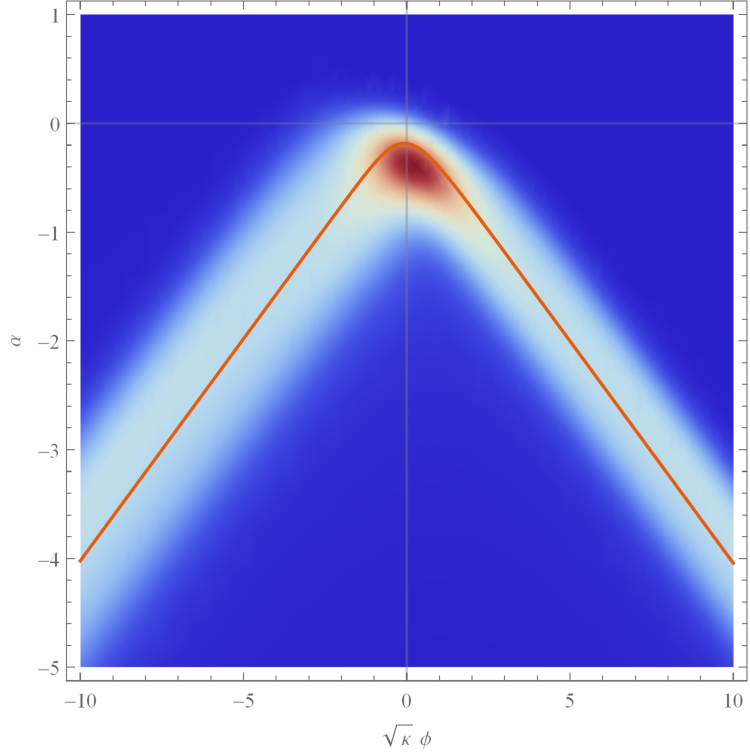
\includegraphics[width=\textwidth]{../plots.paper.nb/naive_cosh_2d.pdf}}
\only<2>{
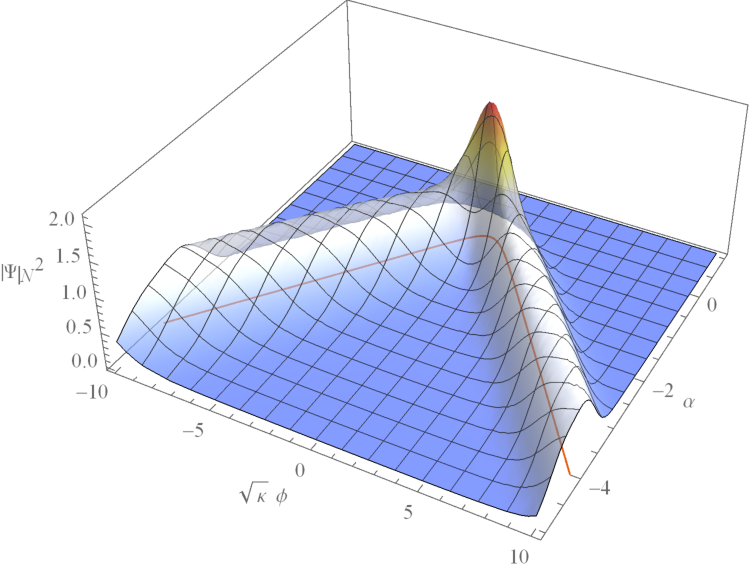
\includegraphics[width=\textwidth]{../plots.paper.nb/naive_cosh_3d.pdf}}
\end{block}
\end{column}
\begin{column}{.49\textwidth}
\begin{block}{Mostafazadeh}
\only<1>{
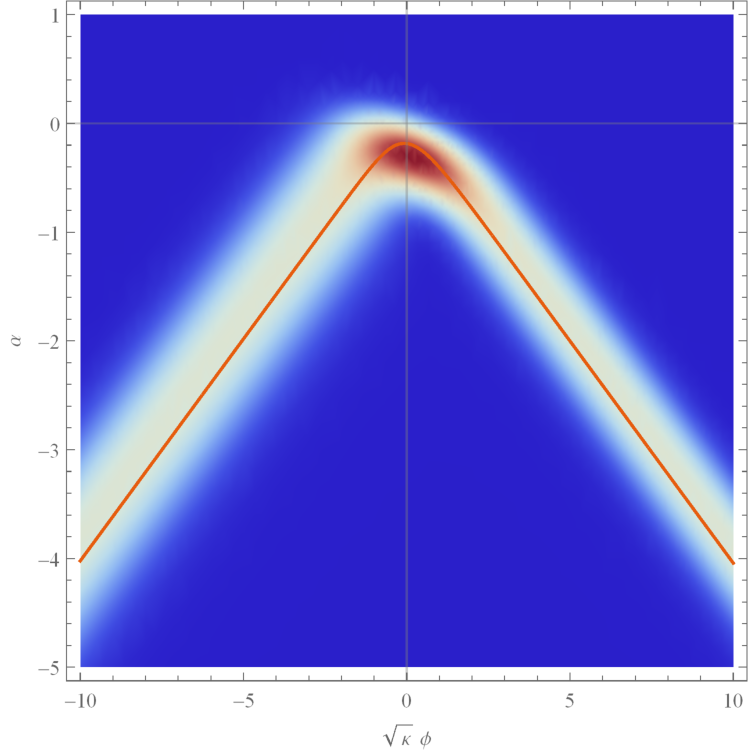
\includegraphics[width=\textwidth]{../plots.paper.nb/mosta_cosh_2d.pdf}}
\only<2>{
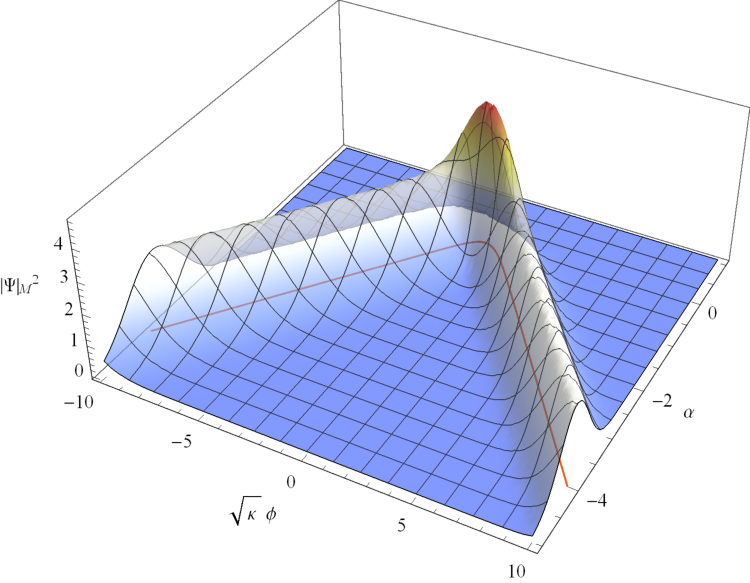
\includegraphics[width=\textwidth]{../plots.paper.nb/mosta_cosh_3d.pdf}}
\end{block}
\end{column}
\end{columns}
\end{frame}

\begin{frame}%
{Wave packets of Gaussian amplitude for quintessence model $\rbr{+,-}$}%
{$\mathrm{F}_{\ii\nu}$, with $\lambda = 4\varkappa^{1/2}/5$,
$V = +\varkappa^{-2}$, $\overline{k}_\beta = -7/2$ and $\sigma_\beta = 7/5$}
\begin{columns}
\begin{column}{.49\textwidth}
\begin{block}{Schrödinger}
\only<1>{
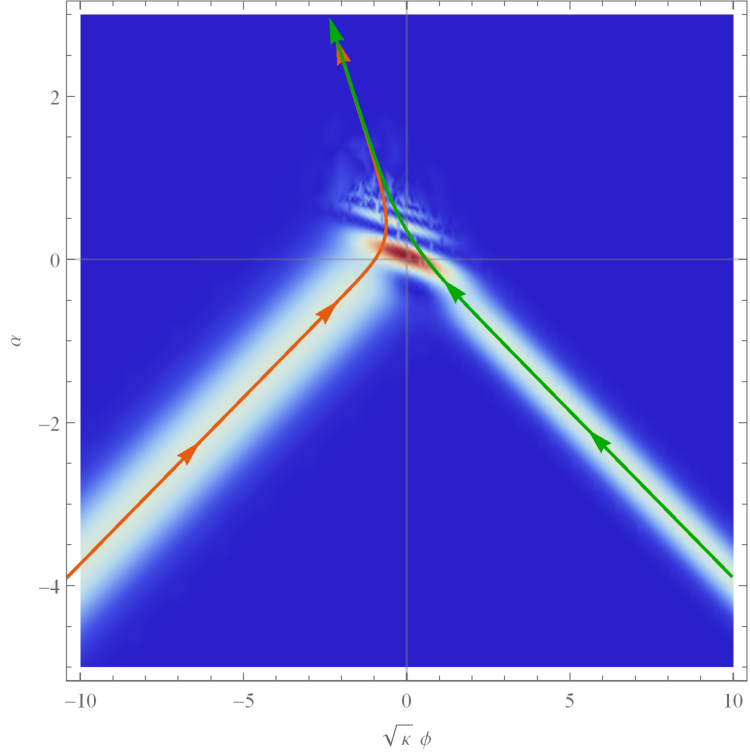
\includegraphics[width=\textwidth]{../plots.paper.nb/naive_sinh_F_2d.pdf}}
\only<2>{
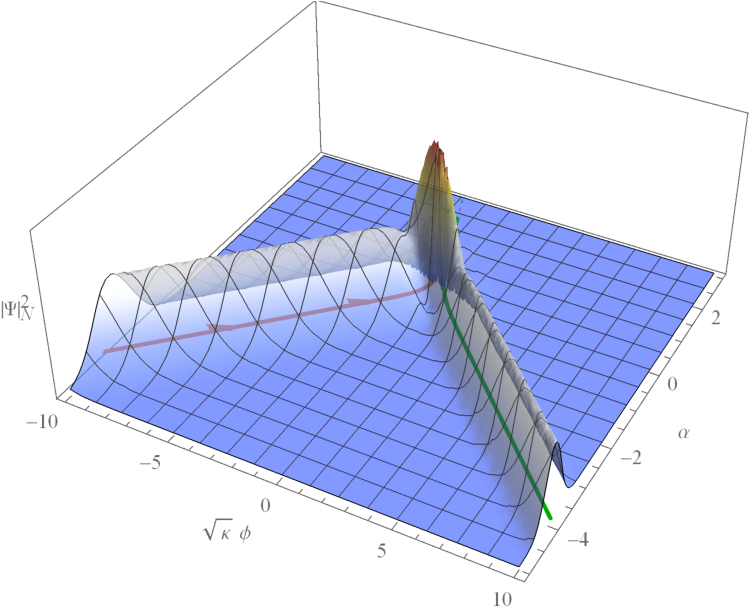
\includegraphics[width=\textwidth]{../plots.paper.nb/naive_sinh_F_3d.pdf}}
\end{block}
\end{column}
\begin{column}{.49\textwidth}
\begin{block}{Mostafazadeh}
\only<1>{
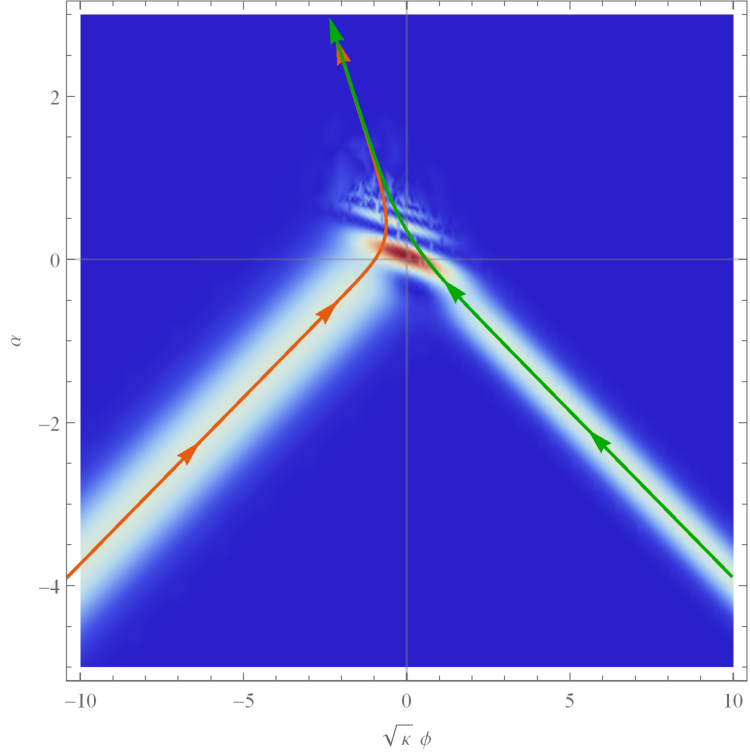
\includegraphics[width=\textwidth]{../plots.paper.nb/mosta_sinh_F_2d.pdf}}
\only<2>{
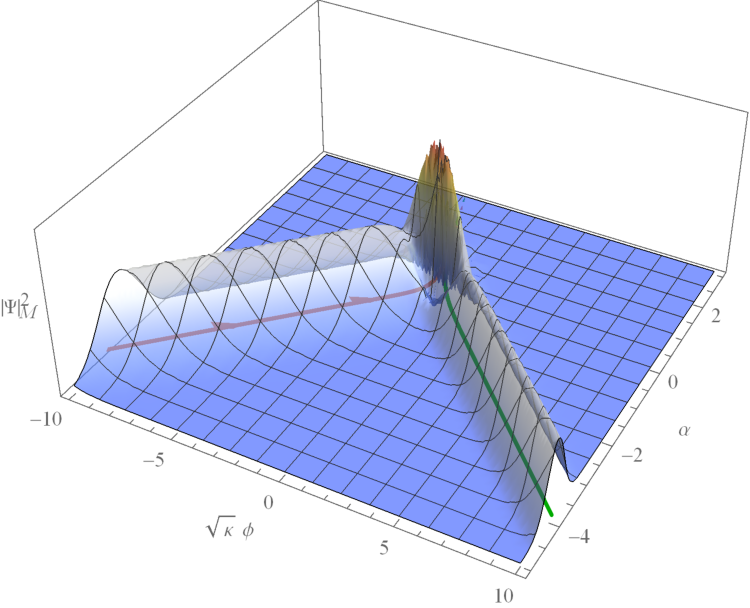
\includegraphics[width=\textwidth]{../plots.paper.nb/mosta_sinh_F_3d.pdf}}
\end{block}
\end{column}
\end{columns}
\end{frame}

\begin{frame}%
{Wave packets of Gaussian amplitude for quintessence model $\rbr{+,-}$}%
{$\mathrm{G}_{\ii\nu}$, with $\lambda = 4\varkappa^{1/2}/5$,
$V = +\varkappa^{-2}$, $\overline{k}_\beta = -7/2$ and $\sigma_\beta = 7/5$}
\begin{columns}
\begin{column}{.49\textwidth}
\begin{block}{Schrödinger}
\only<1>{
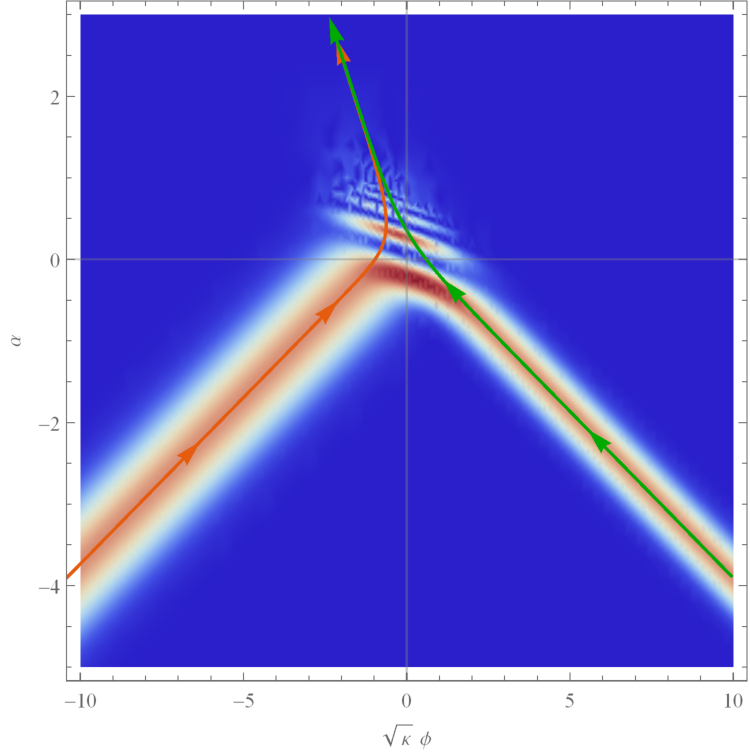
\includegraphics[width=\textwidth]{../plots.paper.nb/naive_sinh_G_2d.pdf}}
\only<2>{
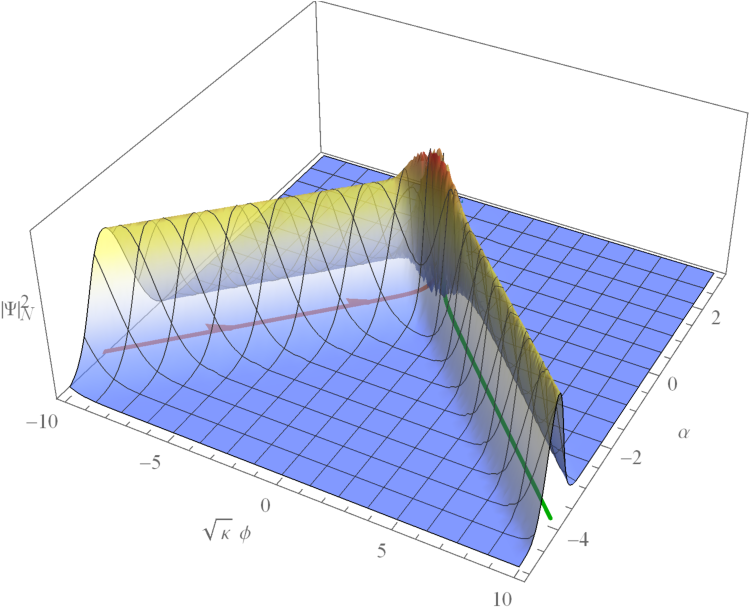
\includegraphics[width=\textwidth]{../plots.paper.nb/naive_sinh_G_3d.pdf}}
\end{block}
\end{column}
\begin{column}{.49\textwidth}
\begin{block}{Mostafazadeh}
\only<1>{
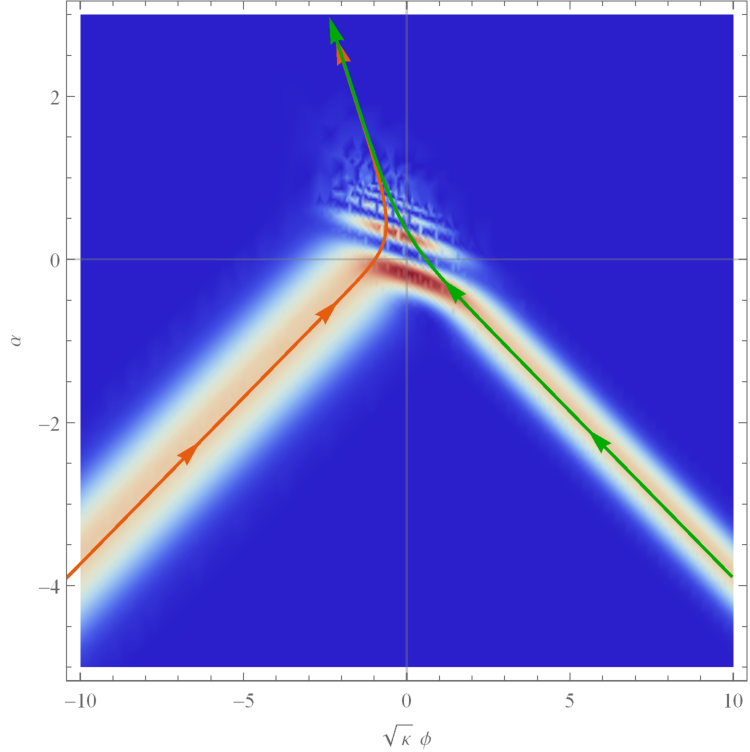
\includegraphics[width=\textwidth]{../plots.paper.nb/mosta_sinh_G_2d.pdf}}
\only<2>{
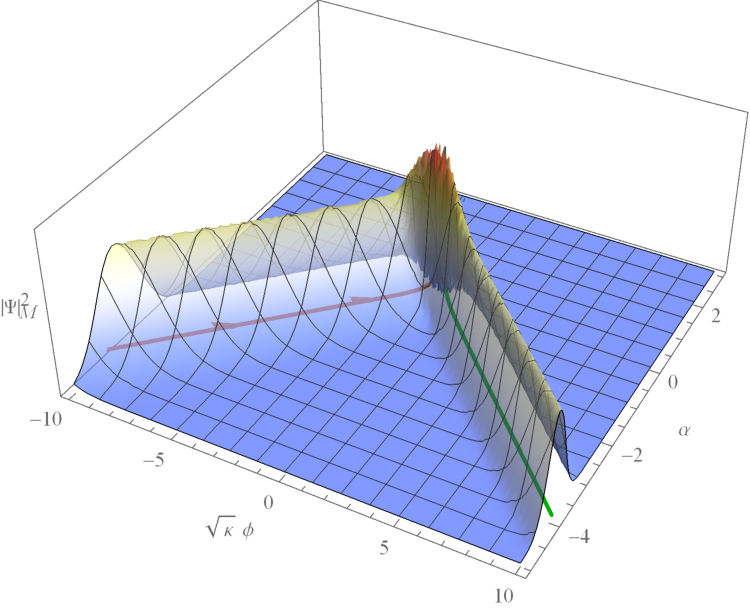
\includegraphics[width=\textwidth]{../plots.paper.nb/mosta_sinh_G_3d.pdf}}
\end{block}
\end{column}
\end{columns}
\end{frame}

\begin{frame}%
{Wave packets with Poissonian amplitude for discrete spectrum}%
{Discrete phantom model $\rbr{-,+}$}
\begin{itemize}
\item Gaussian distribution works for continuous variable

\item For discrete spectrum, one can choose a Poissonian amplitude
\begin{align}
\rfun{A_n}{\overline{n}} \coloneqq
\rbr{\ee^{-\overline{n}}\frac{\overline{n}^n}{n!}}^{1/2}
\end{align}
\item In \footfullcite{Kiefer1990},
$\rfun{A_n}{\overline{n}/\sqrt{2}}$ was chosen.

\end{itemize}
\end{frame}

\begin{frame}%
{Wave packets of Poissonian amplitude for phantom model}%
{$\mathrm{J}_{2n+1}$, with $\lambda = 2\varkappa^{1/2}$,
$V = +\varkappa^{-2}$ and $\overline{k}_\beta = 8$}
\begin{columns}
\begin{column}{.49\textwidth}
\begin{block}{Schrödinger}
\only<1>{
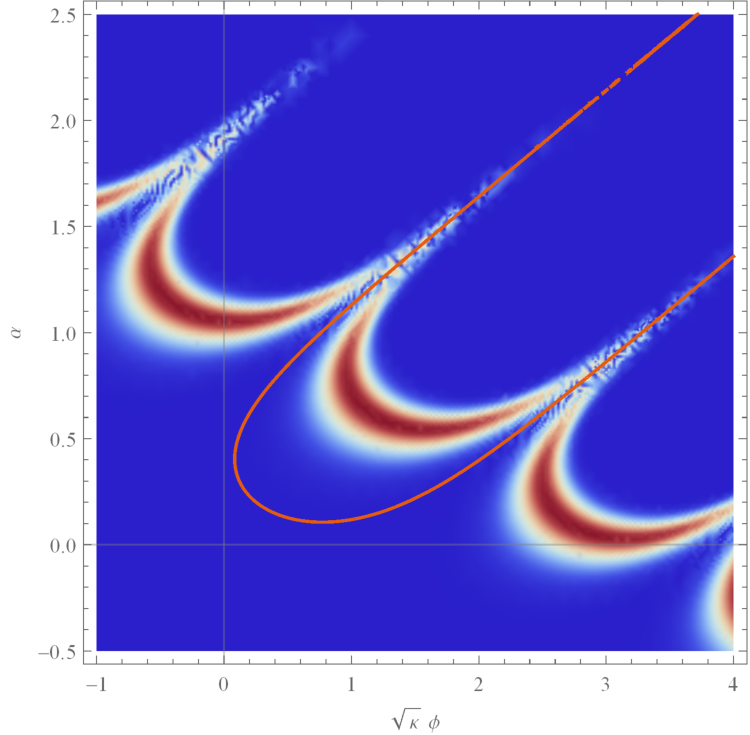
\includegraphics[width=\textwidth]{../plots.paper.nb/naive_cos_1_2d_m.pdf}}
\only<2>{
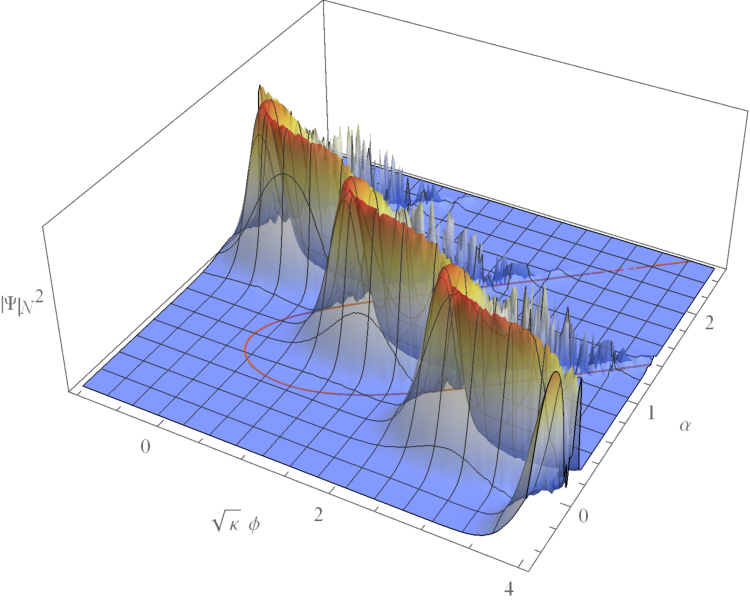
\includegraphics[width=\textwidth]{../plots.paper.nb/naive_cos_1_3d_m.pdf}}
\end{block}
\end{column}
\begin{column}{.49\textwidth}
\begin{block}{Mostafazadeh}
\only<1>{
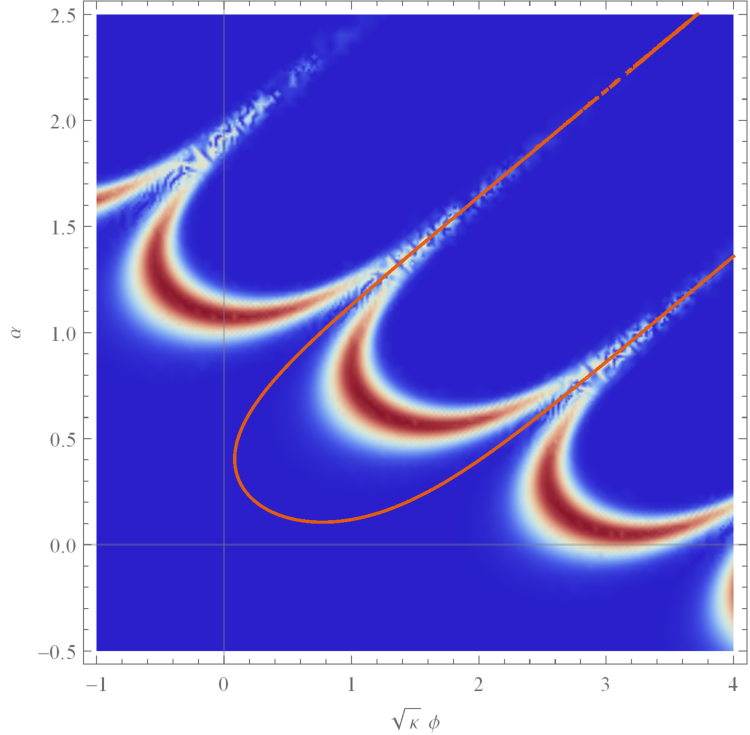
\includegraphics[width=\textwidth]{../plots.paper.nb/mosta_cos_1_2d_m.pdf}}
\only<2>{
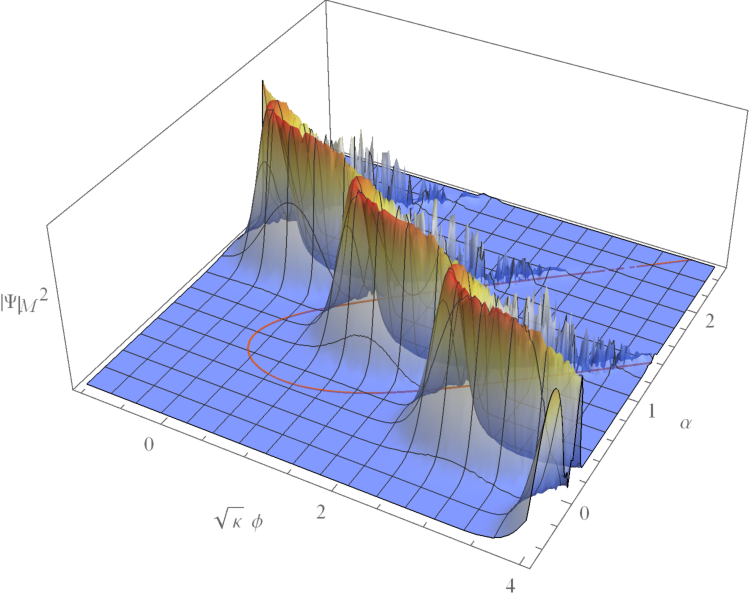
\includegraphics[width=\textwidth]{../plots.paper.nb/mosta_cos_1_3d_m.pdf}}
\end{block}
\end{column}
\end{columns}
\end{frame}

\section{Conclusions}

\begin{frame}%
{Highlights}%
{Revisited}
\begin{itemize}
\item An \alert{integral of motion} was found for the Liouville cosmological
model.
\begin{itemize}
\item Implicit trajectories in minisuperspace were obtained explicitly.
\item The minisuperspace Wheeler--DeWitt equation was integrated exactly.
\end{itemize}
\item The \alert{self-adjointness} of the matter Hamiltonian was found to be 
non-trivial.
\begin{itemize}
\item The degeneracy of the quintessence model $\rbr{+,-}$ was removed.
\item The spectrum of the phantom model $\rbr{-,+}$ became discrete.
\end{itemize}
\item The \alert{semi-classical wave functions} were compared with the 
classical trajectory.
\begin{itemize}
\item Mode functions in the Wentzel--Kramers--Brillouin approximation were 
matched with the classical Hamilton principal function.
\item Semi-classical wave packets were constructed and compared with the 
classical trajectory under the Schrödinger and Mostafazadeh inner product.
\end{itemize}
\end{itemize}
\end{frame}

% \begin{frame}%
% {Issues}%
% %{233}
% \begin{itemize}
% %\item Dimension of wave packets sloppy
% \item In $\rbr{+,-}$ and $\rbr{-,+}$, wave packets contain multiple branches;
% however, the classical universe runs only on one trajectory.
% \item Quantum-corrected $\overline{k}_\beta$ is to be understood.
% \item Wave packets with Gaussian profile are to be constructed, instead of
% inserting Gaussian / Poissonian amplitude artificially.
% \item A normalising $\kappa$ for $\rbr{\cdot,\cdot}_\text{M}^\kappa$ is to be 
% evaluated, otherwise a quantitative comparison of
% $\rbr{\cdot,\cdot}_\text{S}$ and $\rbr{\cdot,\cdot}_\text{M}^\kappa$ is not
% possible.
% \end{itemize}
% \end{frame}

\begin{frame}%
{Outlook}%
%{233}
\begin{itemize}
\item Beyond isotropy: Bianchi models\footfullcite{Kamenshchik2017}

\item Beyond homogeneity: cosmological perturbations 
\footfullcite{Brizuela2016a,Brizuela2016b,Novikov2017,Kamenshchik2018,
Kiefer2018}

\item Beyond single Liouville field: multiple potentials / multiple 
fields\footfullcite{Andrianov2015}

\item Beyond classical matter and Schrödinger inner product: $PT$-symmetric 
field \footfullcite{ANDRIANOV2010,Andrianov2016}

\end{itemize}
\end{frame}


\section*{Appendix}

\subsection*{More trajectories}

\begin{frame}%
{Trajectories for quintessence model $\rbr{+,+}$}%
{$\sech$, with $\beta_0 = 0$, $\vbr{V} = \varkappa^{-2}$ and
$\lambda^2 = 3\varkappa$; varying $p_\beta$}
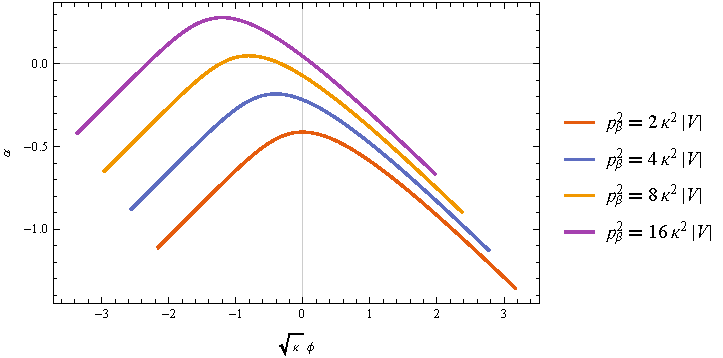
\includegraphics[width=\textwidth]{../plots.nb/sech_pbet.pdf}
\begin{itemize}
	\item has two asymptotes $\chi \propto \pm \beta$
\end{itemize}
\end{frame}

\begin{frame}%
{Trajectories for quintessence model $\rbr{+,+}$}%
{$\sech$, with $\beta_0 = 0$, $\lambda^2 = 3\varkappa$ and
$p_\beta^2 = \varkappa^2\sqrt{\vbr{V}}$; varying $V$}
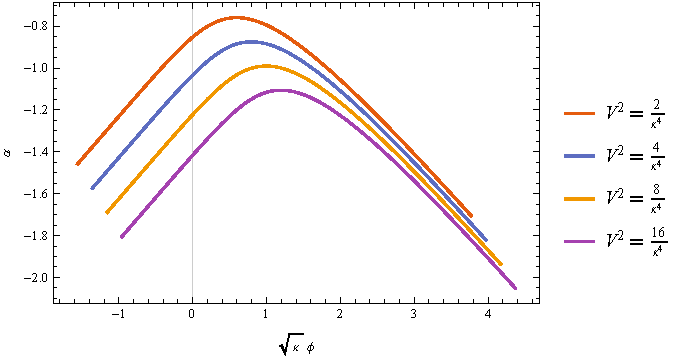
\includegraphics[width=\textwidth]{../plots.nb/sech_Vsqr.pdf}
\begin{itemize}
	\item has two asymptotes $\chi \propto \pm \beta$
\end{itemize}
\end{frame}

% \begin{frame}%
% {Trajectories for quintessence model $\rbr{+,+}$}%
% {$\sech$, with $\beta_0 = 0$, $\lambda^2 = 3\varkappa$ and
% $p_\beta^2 = \varkappa^2\sqrt{\vbr{V}}$; varying $\varkappa$}
% 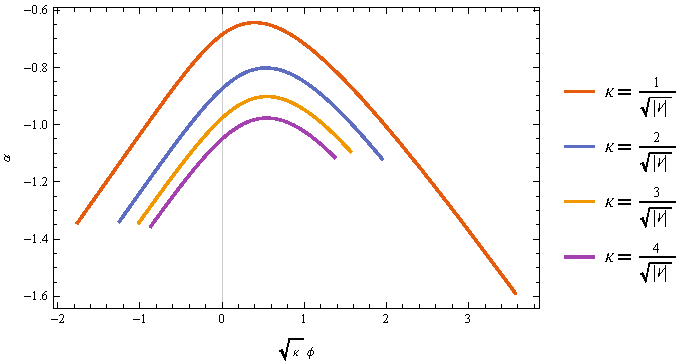
\includegraphics[width=\textwidth]{../plots.nb/sech_vark.pdf}
% \begin{itemize}
% 	\item has two asymptotes $\chi \propto \pm \beta$
% \end{itemize}
% \end{frame}


\begin{frame}%
{Trajectories for quintessence model $\rbr{+,-}$: $\csch$}%
{$\csch$, with $\beta_0 = 0$, $\vbr{V} = \varkappa^{-2}$ and
$p_\beta^2 = \varkappa^2\sqrt{\vbr{V}}$; varying $\lambda$}
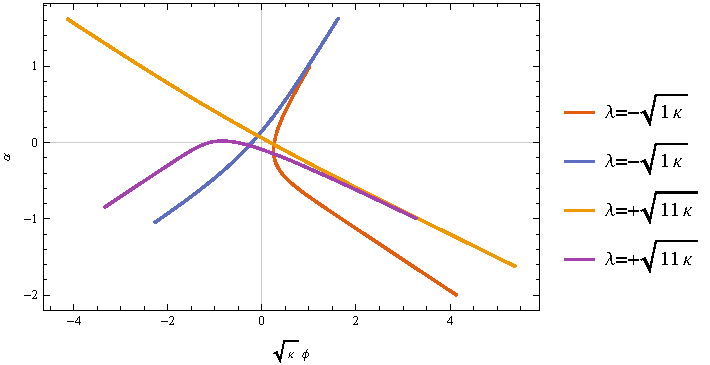
\includegraphics[width=\textwidth]{../plots.nb/csch_lamb_r.pdf}
\begin{itemize}
	\item contains two distinct solutions, separated by $\beta = 0$
	\item has three asymptotes $\chi \propto \pm \beta$ and $\beta = 0$
\end{itemize}
\end{frame}

\begin{frame}%
{Trajectories for quintessence model $\rbr{+,-}$: $\csch$}%
{$\csch$, with $V = \varkappa^{-2}$ and
$\lambda^2 = \varkappa$; varying $p_\beta$}
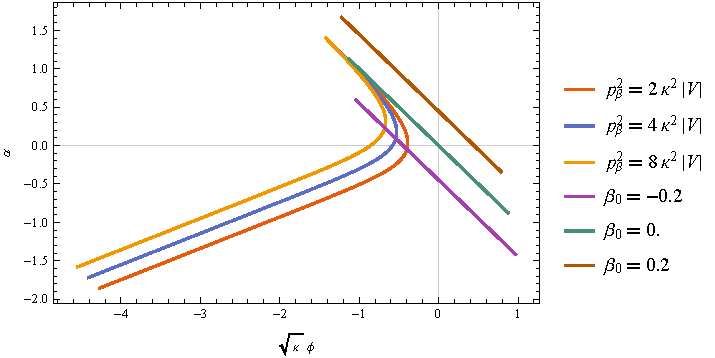
\includegraphics[width=\textwidth]{../plots.nb/csch_pbet_l.pdf}
\begin{itemize}
	\item contains two distinct solutions, separated by $\beta = 0$
	\item has three asymptotes $\chi \propto \pm \beta$ and $\beta = 0$
\end{itemize}
\end{frame}

\begin{frame}%
{Trajectories for phantom model $\rbr{-,+}$}%
{$\sec$, with $V = \varkappa^{-2}$ and
$p_\beta^2 = 3\varkappa^2\sqrt{\vbr{V}}$}
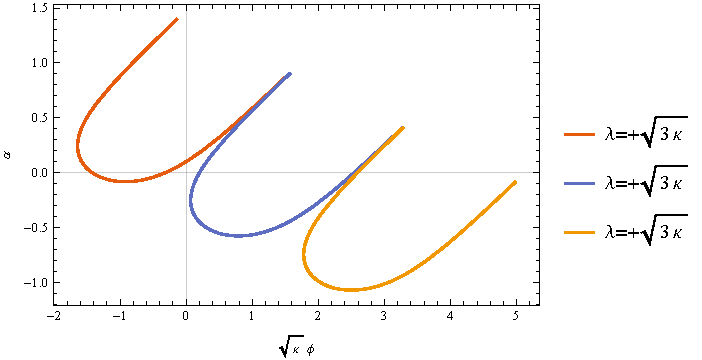
\includegraphics[width=\textwidth]{../plots.nb/csc_lamb_l.pdf}
%\begin{columns}
%\begin{column}{.55\textwidth}
\begin{itemize}
	\item contains infinite distinct solutions
	\item has infinite parallel asymptotes $\beta \propto \rbr{n+1/2}\pp $
\end{itemize}
%\end{column}
%\begin{column}{.4\textwidth}
%\begin{itemize}
%\item is $\beta$-even for $\beta_0 = 0$
%\end{itemize}
%\end{column}
%\end{columns}
\end{frame}

\begin{frame}%
{Trajectories for phantom model $\rbr{-,+}$}%
{$\csc$, with $V = \varkappa^{-2}$ and
$p_\beta^2 = 3\varkappa^2\sqrt{\vbr{V}}$}
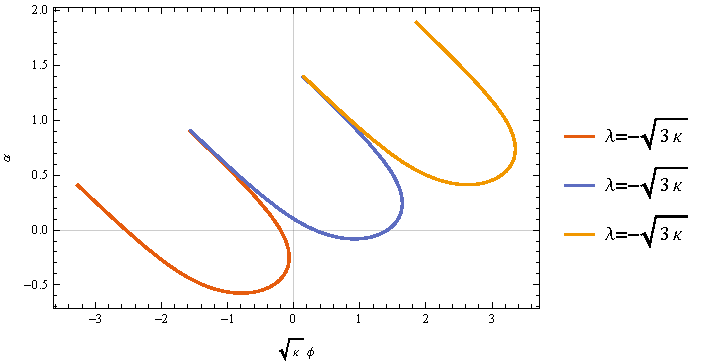
\includegraphics[width=\textwidth]{../plots.nb/csc_lamb_r.pdf}
%\begin{columns}
%\begin{column}{.55\textwidth}
\begin{itemize}
	\item contains infinite distinct solutions
	\item has infinite parallel asymptotes $\beta \propto \rbr{n+1/2}\pp $
\end{itemize}
%\end{column}
%\begin{column}{.4\textwidth}
%\begin{itemize}
%\item is $\beta$-even for $\beta_0 = 0$
%\end{itemize}
%\end{column}
%\end{columns}
\end{frame}

\begin{frame}%
{Trajectories for phantom model $\rbr{-,+}$}%
{$\csc$, with $V = \varkappa^{-2}$ and
$\lambda^2 = 3\varkappa$; varying $p_\beta$}
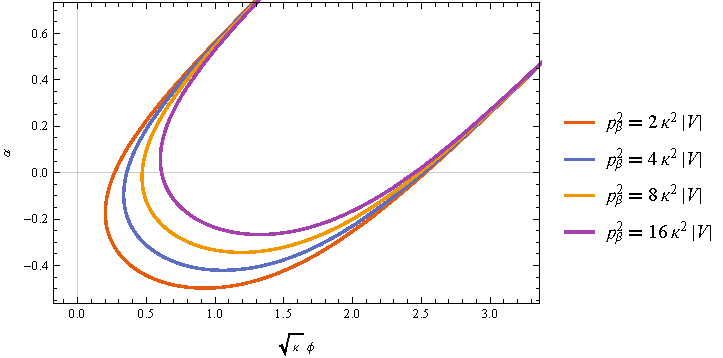
\includegraphics[width=\textwidth]{../plots.nb/csc_pbet_l.pdf}
%\begin{columns}
%\begin{column}{.55\textwidth}
\begin{itemize}
	\item contains infinite distinct solutions
	\item has infinite parallel asymptotes $\beta \propto \rbr{n+1/2}\pp $
\end{itemize}
%\end{column}
%\begin{column}{.4\textwidth}
%\begin{itemize}
%\item is $\beta$-even for $\beta_0 = 0$
%\end{itemize}
%\end{column}
%\end{columns}
\end{frame}

\subsection*{Something else}

\begin{frame}%
{Integration of the transformed first Friedmann equation}%
{General integral for $p_\beta \neq 0$}
In order to integrate the equation under the implicit gauge
\begin{align}
\mscrs\frac{p_\beta^2}{12}\rbr{
-\mscrl\frac{\varkappa^{1/2}}{6}\rbr{\frde{\chi}{\beta}}^2
+\varkappa^{-1/2}}
-\varkappa^{3/2}V\ee^{g\chi} = 0,
\end{align}
one can substitute
\begin{align}
\gamma \coloneqq \sqrt{\frac{3}{2\varkappa}}g\beta, \qquad
\widetilde{\sigma}^2 \coloneqq \frac{p_\beta^2}{12\varkappa^2 \vbr{V}}
\ee^{-g\chi},
\end{align}
to get
\begin{align}
\rbr{\frde{\widetilde{\sigma}}{\gamma}}^2
+\mscrl\rbr{\mscrs\mscrv - \widetilde{\sigma}^2} = 0
\quad\Rightarrow\quad
\frde{\gamma}{\widetilde{\sigma}} = \pm
\frac{1}{\sqrt{\mscrl\rbr{- \mscrs\mscrv + \widetilde{\sigma}^2}}},
\end{align}
which is of the standard inverse hyperbolic / trigonometric form
\textcolor{orange}{except for $\rbr{-,-}$}.
\end{frame}

\begin{frame}%
{Integration of the separated minisuperspace WDW equation}%
%{233}
In order to integrate the separated minisuperspace Wheeler--DeWitt equation
\begin{align}
% \ee^{-\ii k_\beta\beta}\rbr{
% -\mscrl\mscrs\frac{\hslash^2}{2\varkappa^{3/2}}\rfun{\psi''}{\chi}
% -\mscrs\frac{\hslash^2k_\beta^2}{12\varkappa^{1/2}}\rfun{\psi}{\chi}
% +\varkappa^{3/2}V\ee^{g\chi}\rfun{\psi}{\chi}
% } = 0,
\BbbD \rfun{\psi}{\chi} = k_\beta^2 \rfun{\psi}{\chi},\qquad
\BbbD \coloneqq
-\mscrl \frac{6}{\varkappa} \partial_\chi^2
+ \mscrs\mscrv \frac{12\varkappa^2\vbr{V}}{\hslash^2},
%\tag{\ref{eq:separated-10} rev.}
\end{align}
one can transform
\begin{align}
\nu &\coloneqq \sqrt{\frac{2\varkappa}{3}}\frac{k_\beta}{g},\qquad
\sigma^2 \coloneqq 
\frac{8\varkappa^3\vbr{V}\ee^{g\chi}}{\hslash^2 g^2},
%\tag{\ref{eq:trsf-quantum-sigma} rev.}
\end{align}
to get
\begin{align}
\sigma^2\rfun{\psi''}{\sigma}
+\sigma\rfun{\psi'}{\sigma}
+\mscrl\rbr{\nu^2-\mscrs\mscrv\sigma^2}\rfun{\psi}{\sigma} = 0,
\end{align}
which is of the standard Besselian form.
\end{frame}

\subsection*{Self-adjointness}

\begin{frame}%
{Self-adjointness of unbounded operators}%
{General theory}
\begin{itemize}
\item Even in quantum geometrodynamics, the self-adjointness of the matter
Hamiltonian is desirable,
which is typically an unbounded operator in the Hilbert space $\mbfF$ endowed
with the Schr\"odinger inner product $\rbr{\cdot,\cdot}_\text{S}$.

\item Mathematically, an \emph{unbounded} operator
$H$ is characterised not only by its action on a vector, but also by its domain
$\rfun{\mathrm{Dom}}{H} \subsetneq \mbfF$\footfullcite[ch.~9]{hall2013}.

\item In addition to the \emph{symmetricity} $\rbr{H^\dagger \phi_1, \phi_2}
\equiv \rbr{\phi_1, H \phi_2}$, the self-adjointness of an unbounded operator
also requires $\rfun{\mathrm{Dom}}{H^\dagger} = \rfun{\mathrm{Dom}}{H}$.

\item For quantum systems not bounded below, not only the self-adjointness, but
also the symmetricity of the Hamiltonian is not guaranteed automatically.

\item Even when one could find a $\rfun{\mathrm{Dom}_0}{H}$ such that $H$ is
symmetric, one would still be left with $\rfun{\mathrm{Dom}_0}{H^\dagger}
\supseteq \rfun{\mathrm{Dom}_0}{H}$ in general.

\item Sloppily speaking, the process of extending $\rfun{\mathrm{Dom}}{H}$ such
that $\rfun{\mathrm{Dom}}{H^\dagger} = \rfun{\mathrm{Dom}}{H}$ is called
\alert{self-adjoint extension}\footfullcite{Bonneau2001,Araujo2004,%
Essin2006,Gitman2012}; if the extension is unique, the operator is called
\emph{essentially self-adjoint}.

%\item When the self-adjoint extension of the Hamiltonian is not unique, 
\end{itemize}
\end{frame}

% \begin{frame}
%   \frametitle{Allgemeines}

%   \begin{itemize}
%   \item Mit diesem \emph{beamer theme} ist es möglich, Präsentationen in
%     \LaTeX{} mit der Beamer-Klasse zu erstellen, die dem Corporate Design der
%     Universität zu Köln entsprechen
%   \item Auf die Beamer-Klasse wird in diesem Dokument nicht näher eingegangen,
%     nähere Informationen finden Sie unter
%     \url{http://latex-beamer.sourceforge.net/}
%   \end{itemize}

% \end{frame}

%\begin{frame}[fragile]
%  \frametitle{Laden des Themes}
%  \begin{block}{Das Theme kann mit den folgenden Optionen geladen werden}
%    \begin{small}
%\begin{verbatim}
%\usetheme[%
%% uk,      %% Farben aller Fakultaeten
%wiso,     %% Wiso-Fakultaet
%% jura,    %% Rechtswissenschaftliche Fakultaet
%% medizin, %% Medizinische Fakultaet
%% philo,   %% Philosophische Fakultaet
%% matnat,  %% Mathematisch-Naturwissenschaftliche Fakultaet
%% human,   %% Humanwissenschaftliche Fakultaet
%% verw,    %% Universitaetsverwaltung
%%]{UzK}
%\end{verbatim}
%    \end{small}
%
%  \end{block}
%\end{frame}

% \begin{frame}
%   \frametitle{Die Fußzeile}
% 
%   \begin{itemize}
%   \item Es stehen verschiedene Fußzeilen zur Auswahl, die als Option
%     beim Laden des \emph{themes} übergeben werden:
%     \begin{itemize}
%     \item Balken mit allen Fakultätsfarben (Option \texttt{uk})
%     \item Balken in jeweils einer Fakultätsfarbe (Optionen \texttt{wiso, jura,
%         medizin, philo, matnat, human, verw})\footnote{Es werden die 
% offiziellen
%         RGB-Werte aus dem 2-D Handbuch Corporate Design verwendet.}
%     \end{itemize}
%   \item "`Universität zu Köln"' sowie der Name der Fakultät sind im
%     Theme definiert, das Institut oder Seminar kann mit dem Befehl
%     \texttt{\textbackslash institute\{\}} festgelegt werden
%   \item Die Optionen sind im Quellcode dieser Präsentation dokumentiert
%   \end{itemize}

% \end{frame}

% \begin{frame}
%   \frametitle{Englische Präsentationen}
%   \begin{itemize}
%   \item Der Universitäts- sowie die Fakultätsnamen werden
%     standardmäßig auf Deutsch angezeigt.
%   \item Übergeben Sie dem Paket \texttt{babel} die Option
%     \texttt{english}, so werden diese Namen entsprechen angepasst.
%   \item Die Übersetzungen können in der Theme-Datei
%     \texttt{beamerthemeUzK.sty} geändert werden
%   \end{itemize}
% 
% \end{frame}

%\begin{frame}
%  \frametitle{\texttt{block}-Umgebungen}
%  \begin{block}{Standard (\texttt{block})}
%    Verwendet die Farbe "`Blaugrau Mittel"' als Blocktitel-Hintergrund
%  \end{block}
%
%  \begin{exampleblock}{\texttt{exampleblock}}
%    Bei Verwendung der Fußzeile mit allen Fakultätsfarben
%    Titelhintergrund in Wiso-Grün, sonst in der jeweiligen
%    Fakultätsfarbe
%  \end{exampleblock}
%
%  \begin{alertblock}{\texttt{alertblock}}
%    Verwendet das Rot der Folientitel
%  \end{alertblock}
%
%\end{frame}


% \begin{frame}
%   \frametitle{Installation}
%   \begin{itemize}
%   \item Das Theme besteht aus den Dateien
%     \texttt{beamerthemeUzK.sty} und \texttt{beamercolorthemeUzK.sty}
%     sowie den Grafikdateien \texttt{logo.pdf} und
%     \texttt{logo-small.pdf}.
%   \item Das Theme kann auf zwei Arten verwendet werden:
%     \begin{enumerate}
%     \item Die vier Dateien werden in den selben Ordner wie die zu
%       erstellende Präsentation gelegt
%     \item Die vier Dateien werden im lokalen \emph{texmf}-Baum abgelegt
%     \end{enumerate}
%   \item Die zweite Variante ist der ersten vorzuziehen, da das Theme
%     so an einem zentralen Ort vorliegt
%   \end{itemize}
% \end{frame}


% \begin{frame}
%   \frametitle{ToDo}
% 
%   \begin{block}{Was noch zu tun ist\ldots}
%     \begin{itemize}
%     \item Erstellen einer eigenen Titelseite
%     \item \ldots
%     \end{itemize}
%   \end{block}
% 
% \end{frame}

\end{document}
